\clearpage\clearpage
\graphicspath{{sdf/key_management_layer/figures/}}
\acresetall


\section{ETSI QKD 004}
\label{etsi_004}
% Show subsubsections on the Table of Contents
\setcounter{tocdepth}{3}
\setcounter{secnumdepth}{3}

\begin{refsection}
	\begin{tcolorbox}
		\begin{tabular}{p{2.75cm} p{0.2cm} p{10.5cm}}
			\textbf{Goal}          &:& Implementation of the ETSI GS QKD 004\\
			\textbf{Directory}     &:& sdf/dv\_qkd\_ldpc\\
			\textbf{Contributors}   &:& Armando Nolasco Pinto (2021/01/22 - ) \\
									&& Diogo Silva (2021/03/29 - ) \\
		\end{tabular}
	\end{tcolorbox}



\subsection{Introduction}

The security of cryptographic keys negotiated through an insecure communication channel is only ensured by the amount of computational power required to break it, to the point where it becomes unpractical to try to break them. 
This is done with using one-way functions. One-way functions are functions where it is easy to compute its output given a certain input but it is hard to do the reverse process. This makes it so that if someone eavesdrop the key negotiation channel and wants to get the negotiated key they have to test every possibility until they find a match. So if the keys are big enough they are considered secure, although the security of these keys is only assured by the difficulty of the reverse process, which is not mathematically proven. Usually the security of the keys is increased by making them bigger. However, with the presence of quantum computers, these methods become insecure. This is due to quantum computers being very fast at factoring large numbers. Because of this there is a need to create cryptographic key negotiation methods which do not become obsolete in the presence of quantum computers. ETSI Quantum Key Distribution protocol is a method for negotiating cryptographic keys whose security is ensured by the laws of physics, so they cannot be broken either by classic computers or quantum computers. These keys will be negotiated through a quantum channel controlled by specific equipment. The keys can then be distributed to applications via a key management layer which communicates directly with the QKD system. This key management layer is defined in the ETSI QKD 004 standard. 

\subsection{Key Management Layer}

Although the QKD system manages the exchange of cryptographic keys, those keys need to be distributed and synced with the various applications that will use them. This is done by the Key Management Layer. This layer will ensure that the applications that communicate with each other at both ends use the same cryptographic key. The Key Management Layer provides the applications with an API (Application Programming Interface) for them to interact with the QKD System. The interface must have the following functions: 

\begin{lstlisting}
	OPEN_CONNECT(in source, in destination, inout QoS, inout Key_stream_ID, out status)
	GET_KEY(in Key_stream_ID, inout index, out Key_buffer, inout Metadata, out status)
	CLOSE(in Key_stream_ID, out status)
\end{lstlisting}

\pagebreak

\begin{itemize}
	
	\item\underline{OPEN\textunderscore CONNECT(in source, in destination, inout QoS, inout Key\textunderscore stream\textunderscore ID, out status)}
	
		This function associates a Key\textunderscore stream\textunderscore ID to a set of future keys at both ends of the QKD system and establishes a set of parameters for the key service specified by the QoS structure. This function blocks until the peers are connected or the Timeout value is exceeded.
	
	\item\underline{GET\textunderscore KEY(in Key\textunderscore stream\textunderscore ID, inout index, out Key\textunderscore buffer, inout Metadata, out status)}
	
		This function returns the required amount of key material requested for this specific Key\textunderscore stream\textunderscore ID. In case it does not return the key material it should return a error message. The QKD Management Layer should return an index value for the specified key. This index is used for synchronization purposes. The key position will be the result of multiplying the index value by the Key\textunderscore chunk\textunderscore size value. 
		
	\item\underline{CLOSE(in Key\textunderscore stream\textunderscore ID, out status)}
	
		This function verifies if the QKD link is available and the key\textunderscore handle association is synchronized at both ends of the link. This function does not block and thus returns immediately indicating if both sides of the link are synchronized or if an error has occurred.
			
\end{itemize}

\subsubsection{Parameters}

The parameters used by the API functions are the following:

\begin{lstlisting}
	Key_stream_ID
	Key_buffer
	Index
	Source
	Destination
	QoS
	Metadata
	Status
\end{lstlisting}

\begin{itemize}
	
	\item\underline{Key\textunderscore stream\textunderscore ID}
		
		The Key\textunderscore stream\textunderscore ID is a unique identifierfor the group of bits provided by the QKD Key Manager to the application. It is a 16 bytes UUID (Universally unique identifier).
	
	\item\underline{Key\textunderscore buffer}
	
		The key\textunderscore buffer is a buffer containing the current stream of keys. It should be stored as an array of bytes.
		
	\item\underline{Index}
	
		Position of the key to be accessed within the reserved key store for the application. Should be stored as a 32 bit unsigned integer
		
	\item\underline{Source}
	
		Identifier of the source application connection to the QKD key management layer. The identifier is structured as an URI.
		
	\item\underline{Destination}
	
		Identifier of the destination application connecting to the QKD key management layer. The identifier is structured as an URI.
		
	\item\underline{QoS}
	
		The QoS parameters is a structure composed by the following parameters:
		
		\begin{itemize}
			\item{Key\textunderscore chunk\textunderscore size}
				
				Length of the key buffer requested by the application. 32 bit unsigned integer.
				
			\item{Max\textunderscore bps}
			
				Maximum key rate requested in bits per seconds. 32 bit unsigned integer.
				
			\item{Min\textunderscore bps}
			
				Minimum key rate requested in bits per seconds. 32 bit unsigned integer.
				
			\item{Jitter}
				
				Maximum expected deviation, in bps, for key delivery. 32 bit unsigned integer.
				
			\item{TTL (Time to Live)}
			
				Time after which the keys corresponding to this Key\textunderscore stream\textunderscore ID shall be erased. 32 bit unsigned integer.
				
			\item{Metadata mimetype}
			
				Field that defines the format of the metadata on each subsequent GET\textunderscore KEY call. Char array of size 256.
				
		\end{itemize}
	
	\item\underline{Metadata}
		
		\begin{itemize}
			\item{Metadata\textunderscore size}
				Size of metadata buffer in characters. 32 bit unsigned integer.
				
			\item{Metadata\textunderscore buffer}
				Buffer for the returned metadata.

		\end{itemize}
		
	\item\underline{status}
	
		32 bit unsigned integer that indicates the success or failure of the request. The output values are the following:
		
		\begin{itemize}
			\item{0: }
				Successful
			\item{1: }
				Successful connection, but peer not connected.
			\item{2: }
				QKD\textunderscore GET\textunderscore KEY failed because insufficient key available.
			\item{3: }
				QKD\textunderscore GET\textunderscore KEY failed because peer application is not yet connected.
			\item{4: }
				No QKD connection available.
			\item{5: }
				OPEN\textunderscore CONNECT failed because the Key\textunderscore stream\textunderscore ID is already in use.
			\item{6: }
				TIMEOUT\textunderscore ERROR. The timeout has been exceeded.
			\item{7: }
				OPEN failed because requested QoS settings could not be met, counter proposal included in return has occurred.
			\item{8: }
				GET\textunderscore KEY failed because metadata field size insufficient. Returned Metadata\textunderscore size value holds minimum needed size of metadata.
		\end{itemize}
			
\end{itemize}

\subsubsection{Notes}

Some additional considerations to be taken into account are:
\begin{itemize}
	\item
		An application may request various different keys and there is no limit to the number of key streams a given application can request. The only requirement is that the Key\textunderscore stream\textunderscore ID must be different. 
	\item
		The Key\textunderscore stream\textunderscore ID must uniquely identify the key material and the key material cannot be derived from it.
	\item
		The Key\textunderscore stream\textunderscore ID may or may not be provided by the application. In case the application does not provide a Key\textunderscore stream\textunderscore ID the Key Management Layer should generate one and return it to the application.
\end{itemize}

\subsection{Extending QKD to oblivious keys}

ETSIs QKD protocol could be extended to use oblivious keys instead. For that we need to add API calls that deal with QOKD instead of QKD.

\begin{lstlisting}
	QOKD_OPEN_CONNECT(in source, in destination, inout QoS, inout Key_stream_ID, out status)
	QOKD_GET_KEY(in Key_stream_ID, inout index, out Key_buffer, inout Metadata, out status)
	QOKD_CLOSE(in Key_stream_ID, out status)
\end{lstlisting}

There is also a additional parameter needed, \texttt{role} , that serves the purpose of indicating if the application will play the role of Alice or Bob in the oblivious transfer because both parties follow different routines in the transfer and the Key Manager needs that information. 
The status parameter may return an additional error, \texttt{1024}, that indicates conflicting roles, in case both APPA and APPB try to play the same role in the OT.

\subsection{Use Case Examples}

\begin{itemize}
	\item
	APPA: Application at host A
	\item
	APPB: Application at host B
	\item
	KMA: QKD key manager at host A
	\item
	KMB: QKD key manager at host B
	\item
	QKSA: QKD system at host A
	\item
	QKSB: QKD system at host B
\end{itemize}

\subsubsection{QKD with undefined key\textunderscore handle}

\begin{figure}[H]
	\centering
	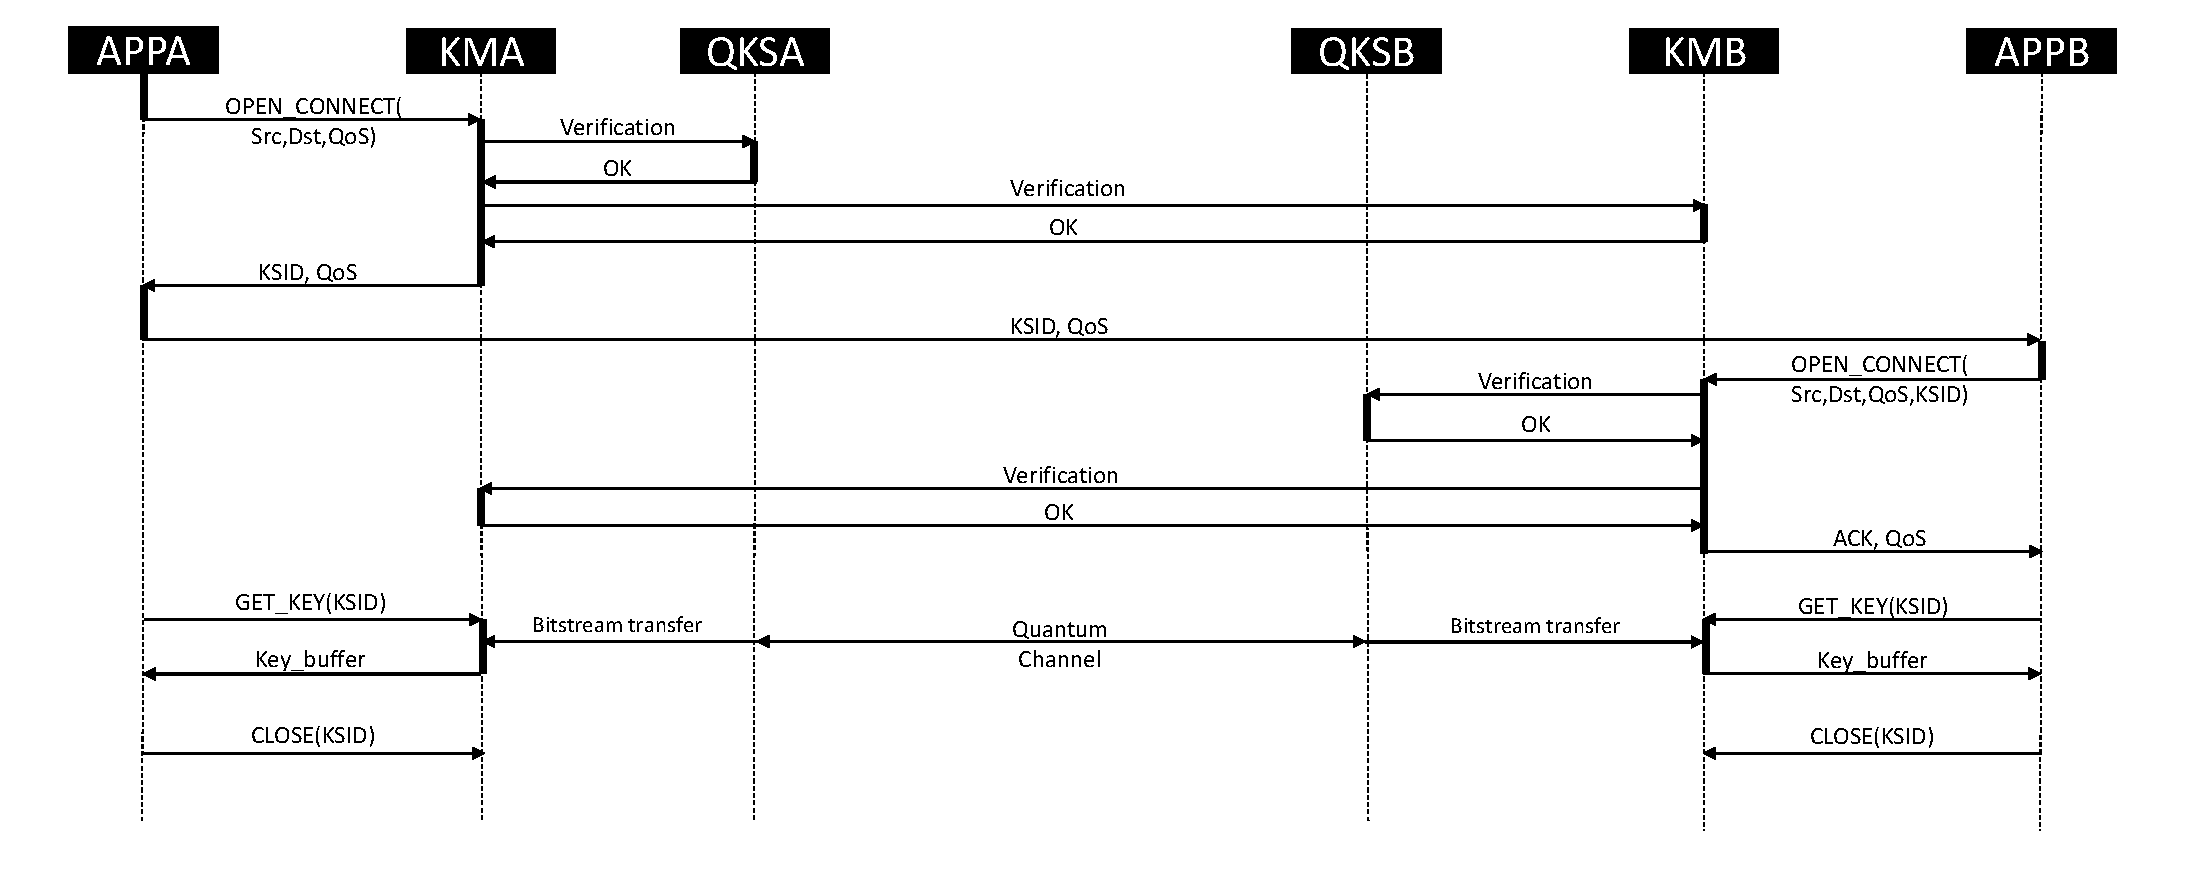
\includegraphics[width=15cm]{qkdUpdated.pdf}
	\caption{QKD with undefined Key\textunderscore stream\textunderscore ID}
	\label{fig:QKDUndefinedKSID}
\end{figure}

In this example APPA does not provide a Key\textunderscore stream\textunderscore ID. Because of that the Key Manager returns a generated Key\textunderscore stream\textunderscore ID, which the application has to send to the APPB to make sure that the KSID is synchronized at both ends.

\subsection{Block Diagram}

%\begin{figure}[H]
%	\centering
%	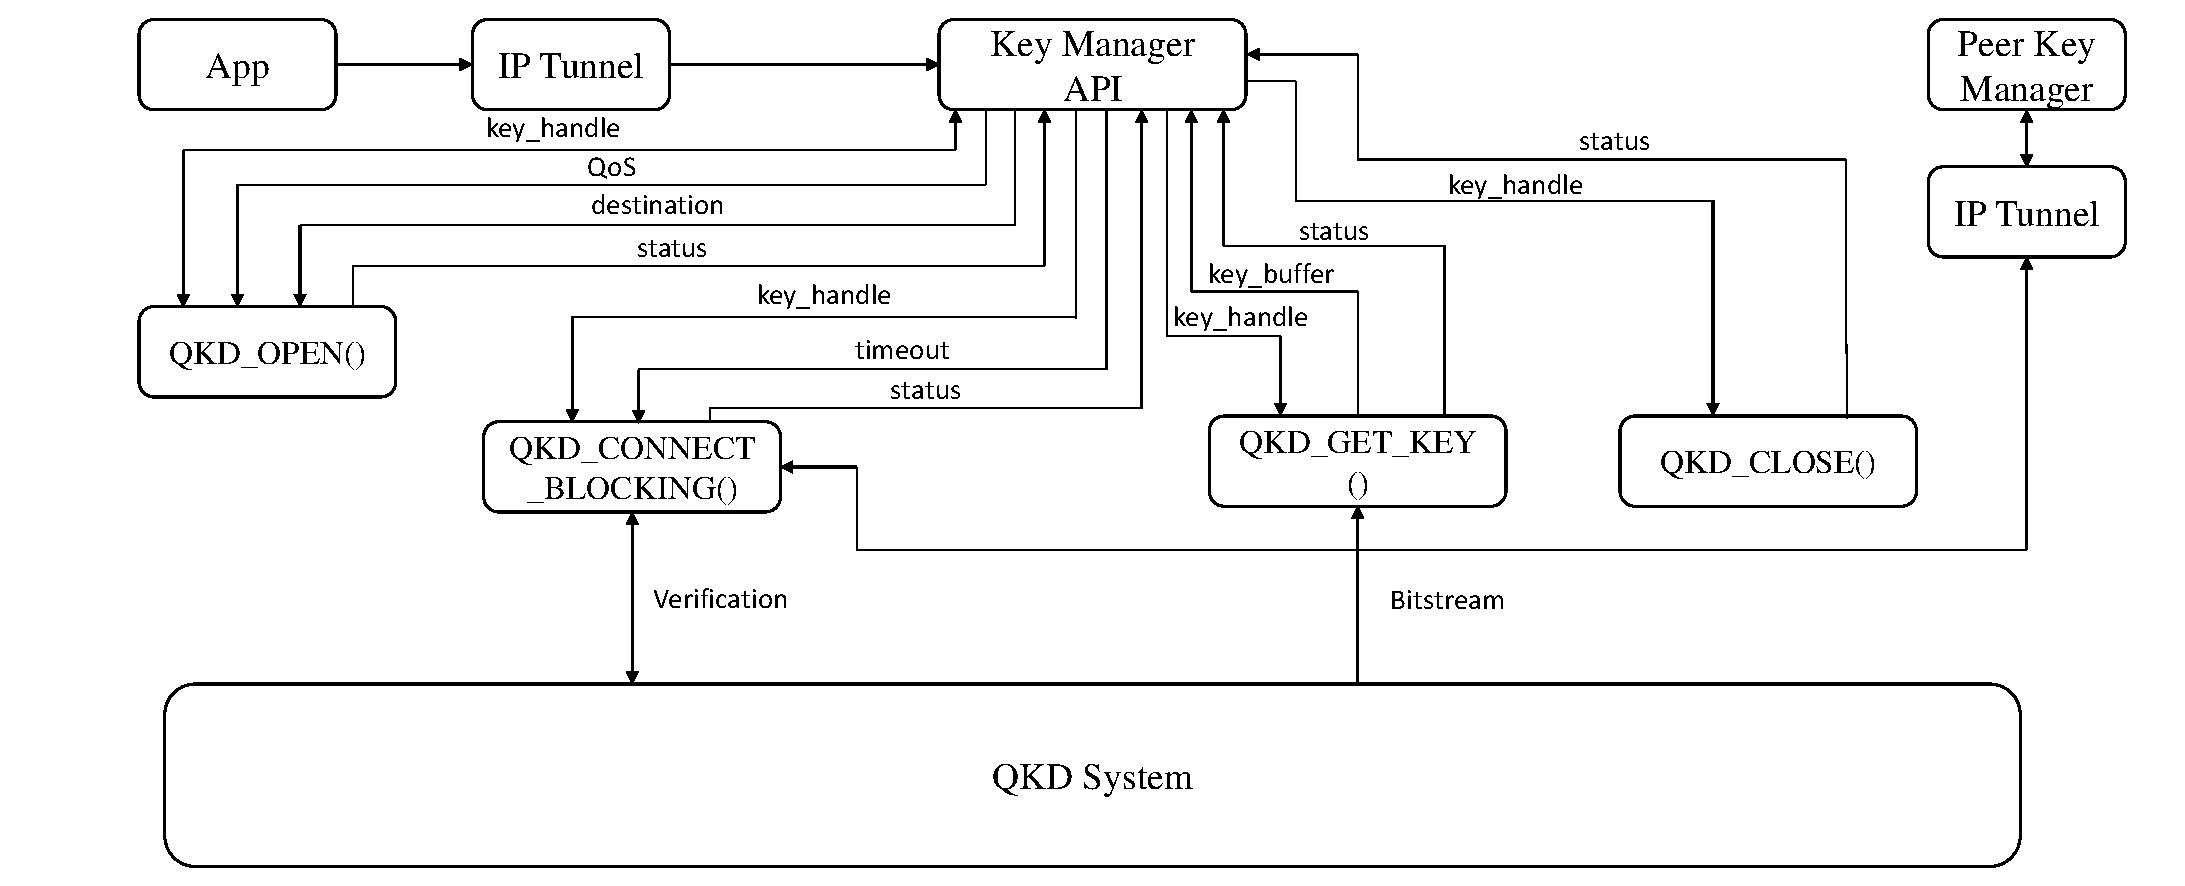
\includegraphics[width=15cm]{blockDiagram.pdf}
%	\caption{Block Diagram}
%	\label{fig:blockDiagram}
%\end{figure}

%\begin{figure}[H]
%	\centering
%	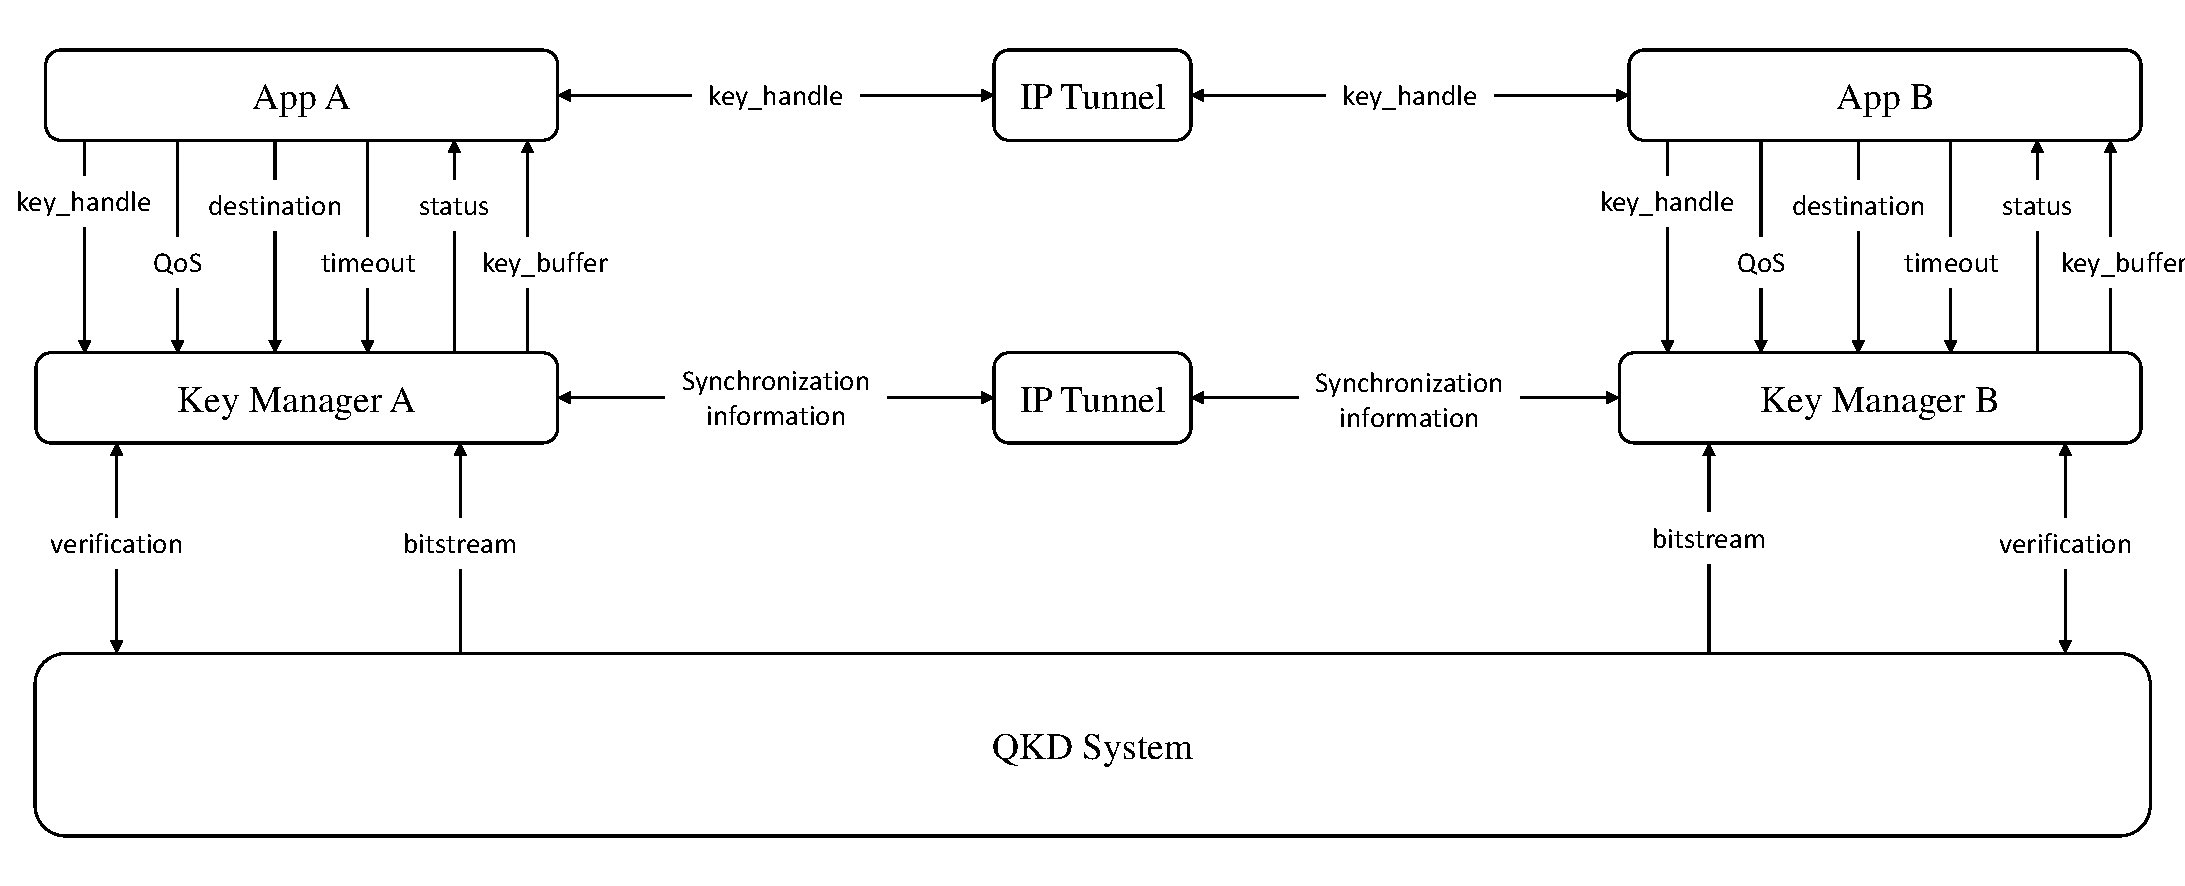
\includegraphics[width=15cm]{blockDiagram2.pdf}
%	\caption{Block Diagram 2}
%	\label{fig:blockDiagram2}
%\end{figure}

\begin{figure}[H]
	\centering
	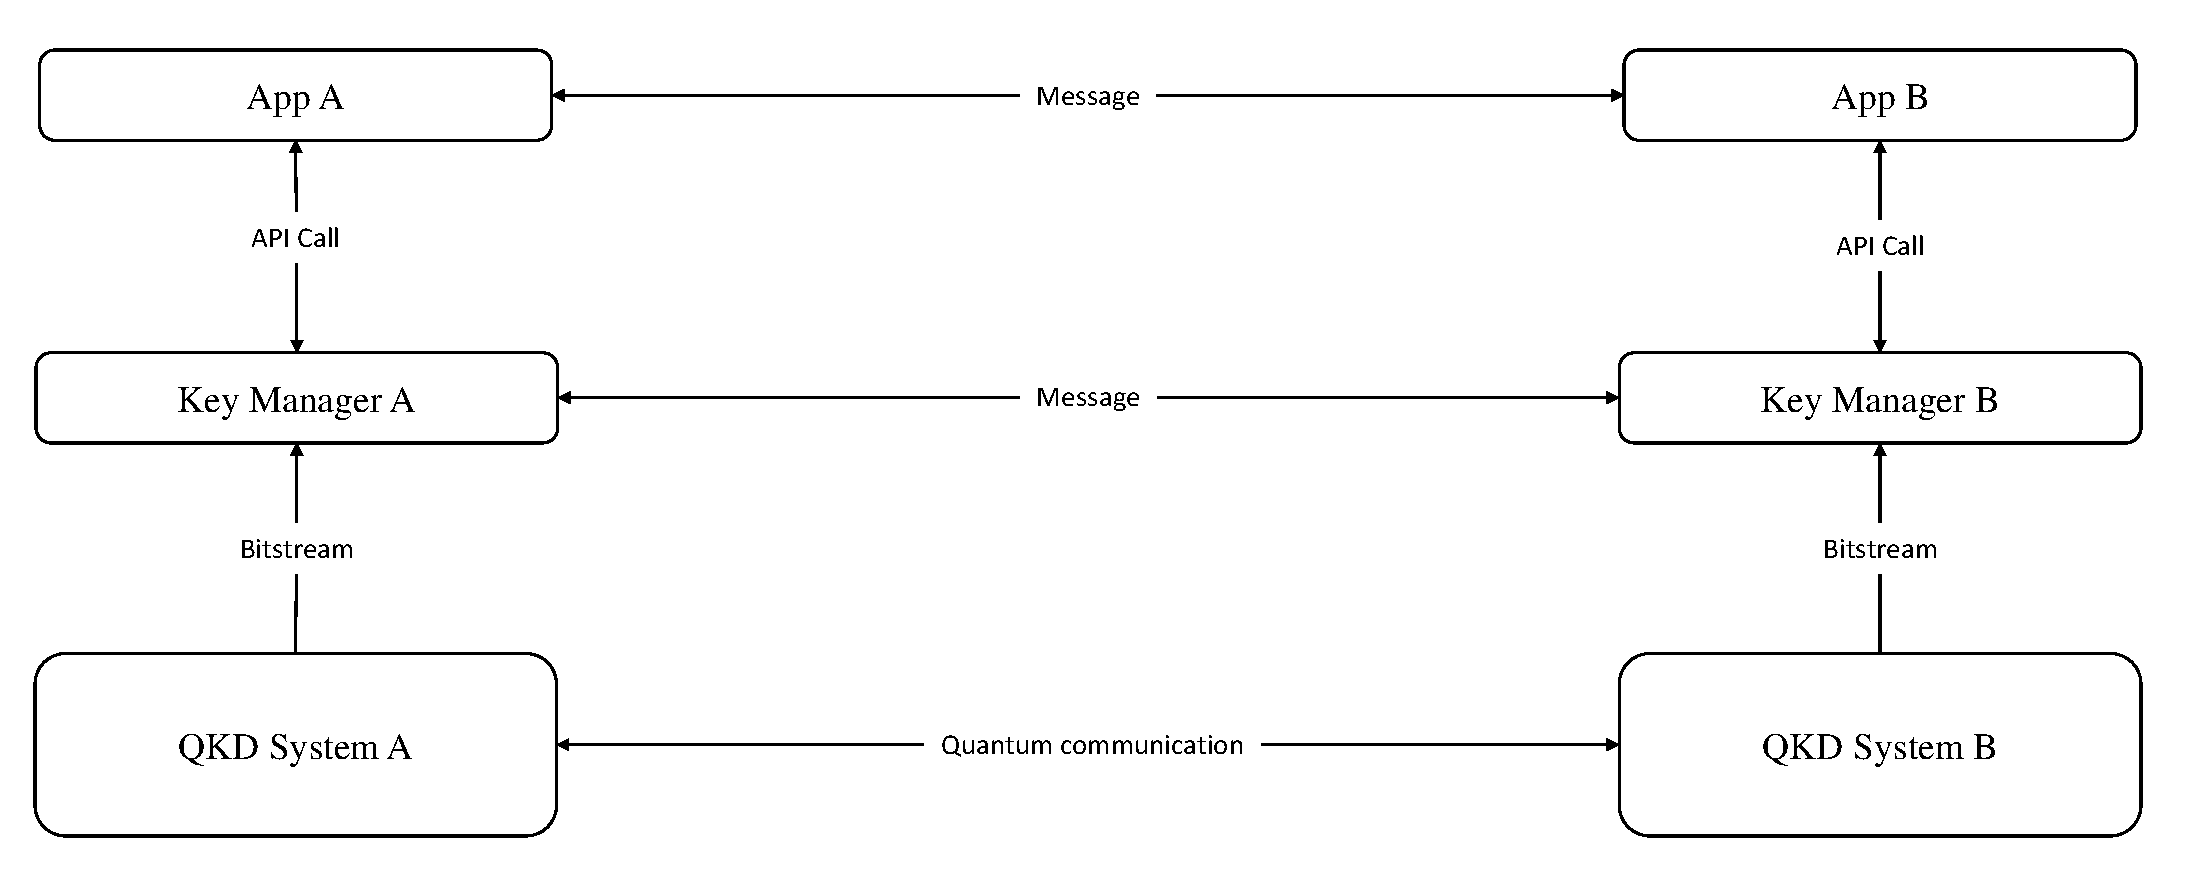
\includegraphics[width=15cm]{communicationsBlockDiagram.pdf}
	\caption{Communications Block Diagram}
	\label{fig:blockDiagram3}
\end{figure}

The objective of this system is to provide the same symmetric and oblivious keys to both applications (APP A and APP B). These keys will come from the QKD systems. The Key Management Layer is responsible to get the keys from the physical QKD system. From there there is a need for the Key Manager to communicate with its peer Key Manager for key synchronization purposes. The way this is done is left to the implementer. One simple example is a socket communication. From there both Apps need to get the keys from their respective Key Manager. This should be done through calls to an API. The technology used for this API is left to the implementer. Two examples of ways to implement this API are REST and a socket. The only requirement is that the API accepts data in json format. The communication between both Apps is left to the implementer. This need for this communication is to make sure that both Apps have the same Key\textunderscore stream\textunderscore ID.

\begin{figure}[H]
	\centering
	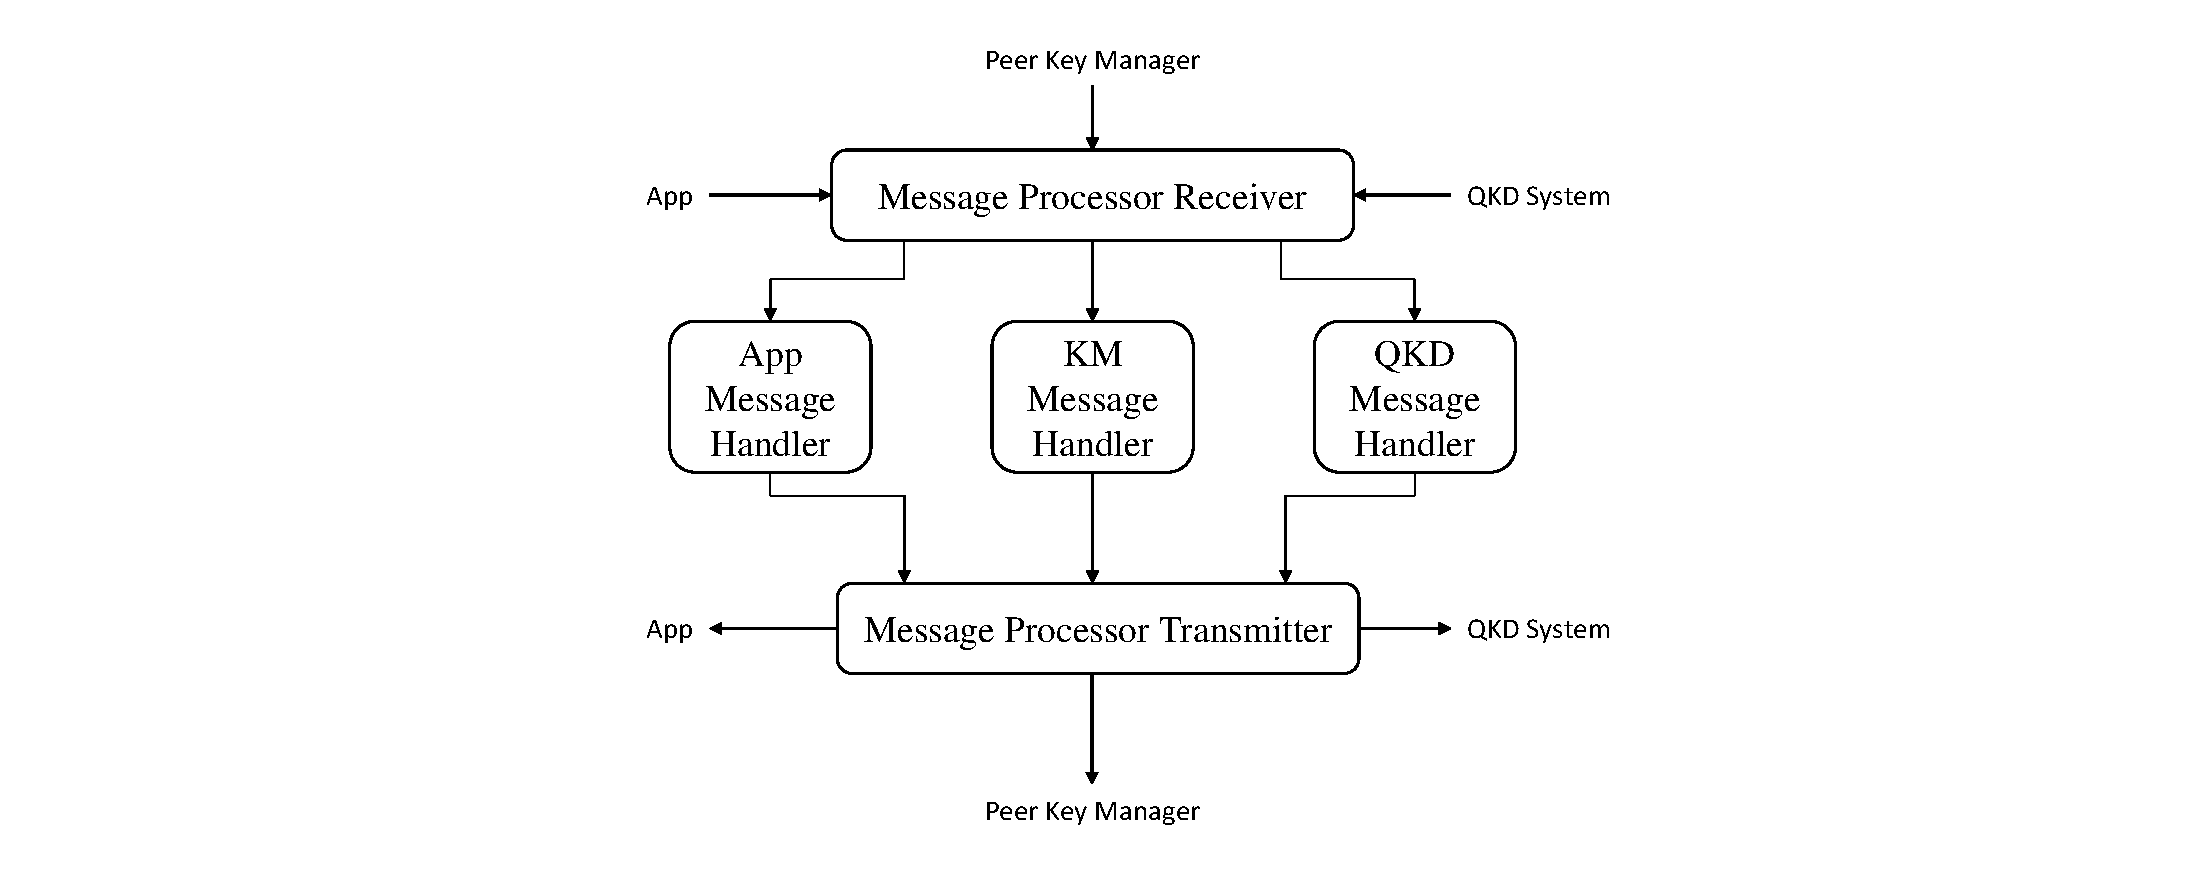
\includegraphics[width=15cm]{messageProcessor.pdf}
	\caption{Message Processor}
	\label{fig:blockDiagram4}
\end{figure}

Above is a simple diagram that illustrates the message processor of each Key Manager. The Receiver gets its input from the App, the Peer Key Manager and the QKD System. These inputs might come in different formats. The receiver than relays that information to the appropriate message handler, depending on who the input came from. Once the handlers have processed the information and return an answer, that information is send to the Message Processor Transmitter, whose job is to then send the response to the adequate system.

\subsection{Madrid Example}

A example was provided from our partners in Madrid. This example is written in Python 3.6. It is a generic 004 implementation that has no hardware connection to the QKD system, and so it simulates it by generating a random key. There is a script that simulates two applications exchanging messages encrypted with the keys provided by the LKMS. The LMKS's can be run without the applications and used with our own application.

\subsection{Socket Description}

\begin{figure}[H]
	\centering
	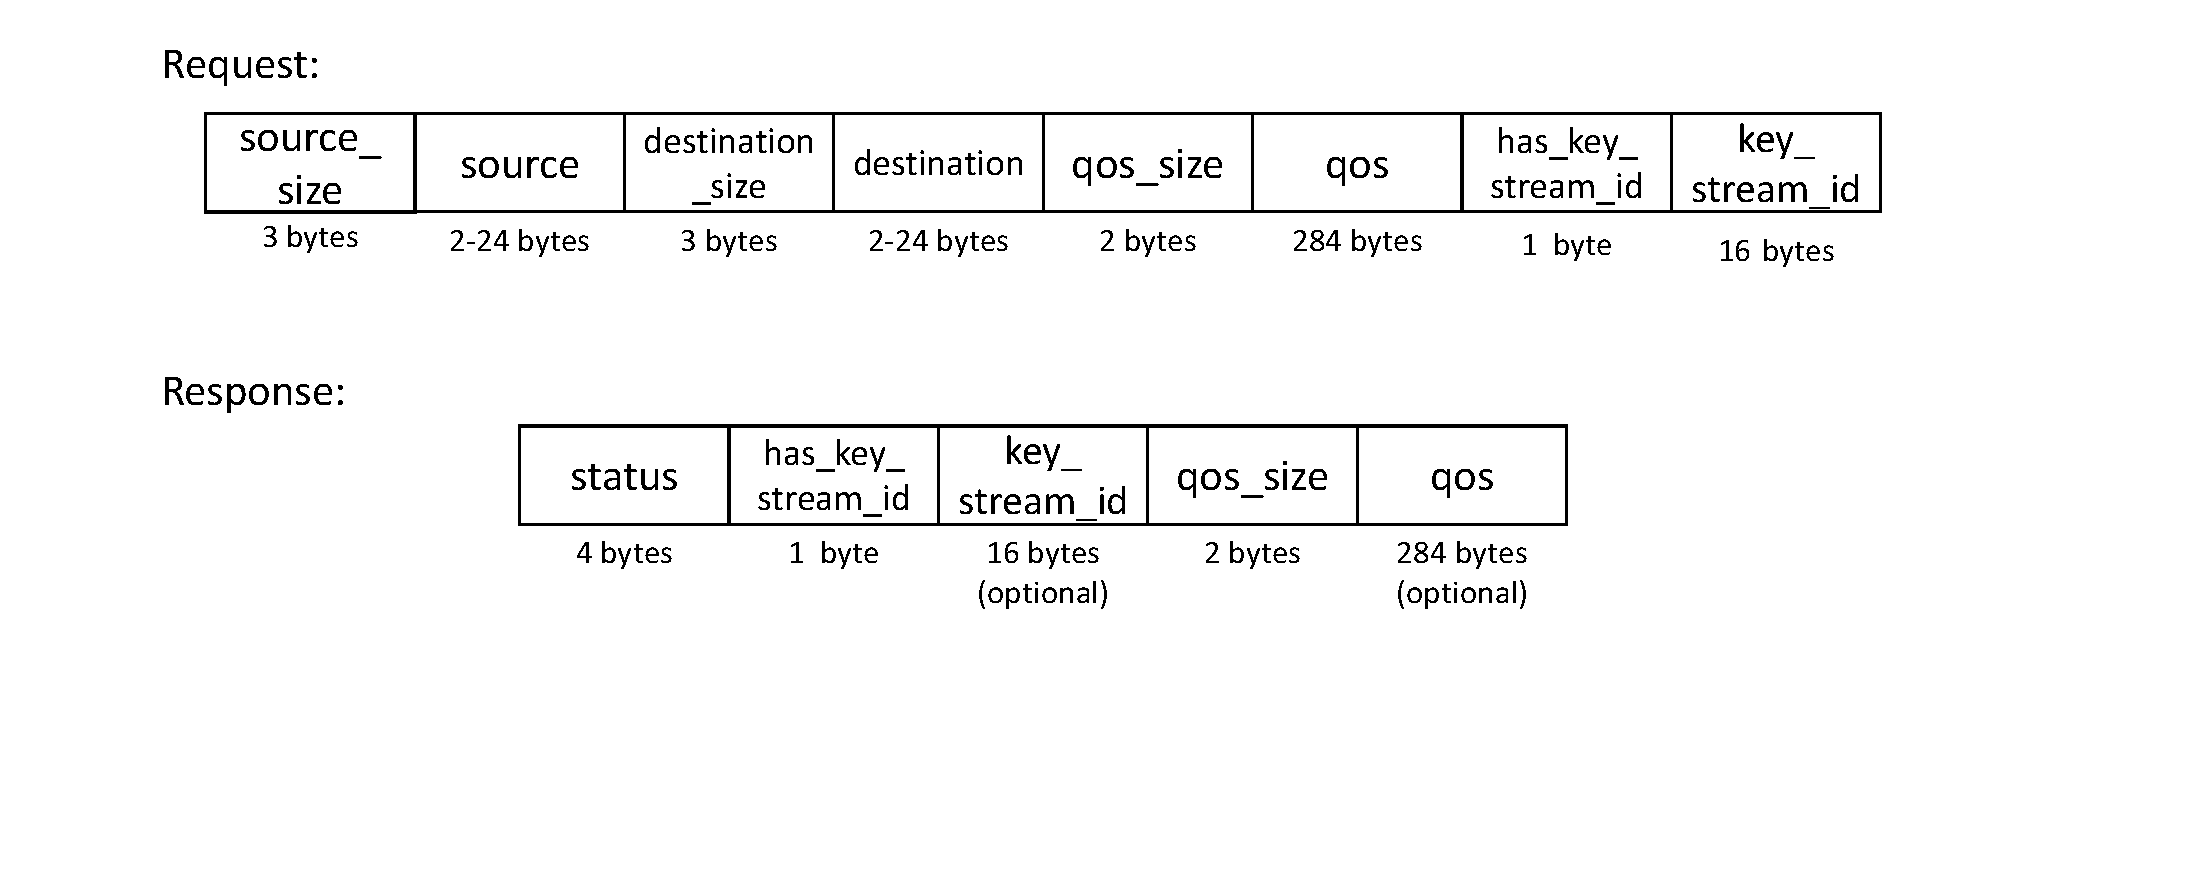
\includegraphics[width=15cm]{open_connect_socket.pdf}
	\caption{Open Connect Socket}
	\label{fig:openConn}
\end{figure}

\begin{itemize}
	\item\underline{source}
		
		URI of the source

	\item\underline{source\textunderscore size}

		Size of the source URI

	\item\underline{destination}

		URI of the destination

	\item\underline{destination\textunderscore size}

		Size of the destination URI

	\item\underline{qos\textunderscore size}

		Size of the QoS structure

	\item\underline{qos}

		QoS structure

	\item\underline{has\textunderscore key\textunderscore stream\textunderscore id}

		Informs if the request provides a KSID

	\item\underline{key\textunderscore stream\textunderscore id}

		KSID provided by the application (optional)

	\item\underline{status}

		Status code returned by the KMS

\end{itemize}

\begin{figure}[H]
	\centering
	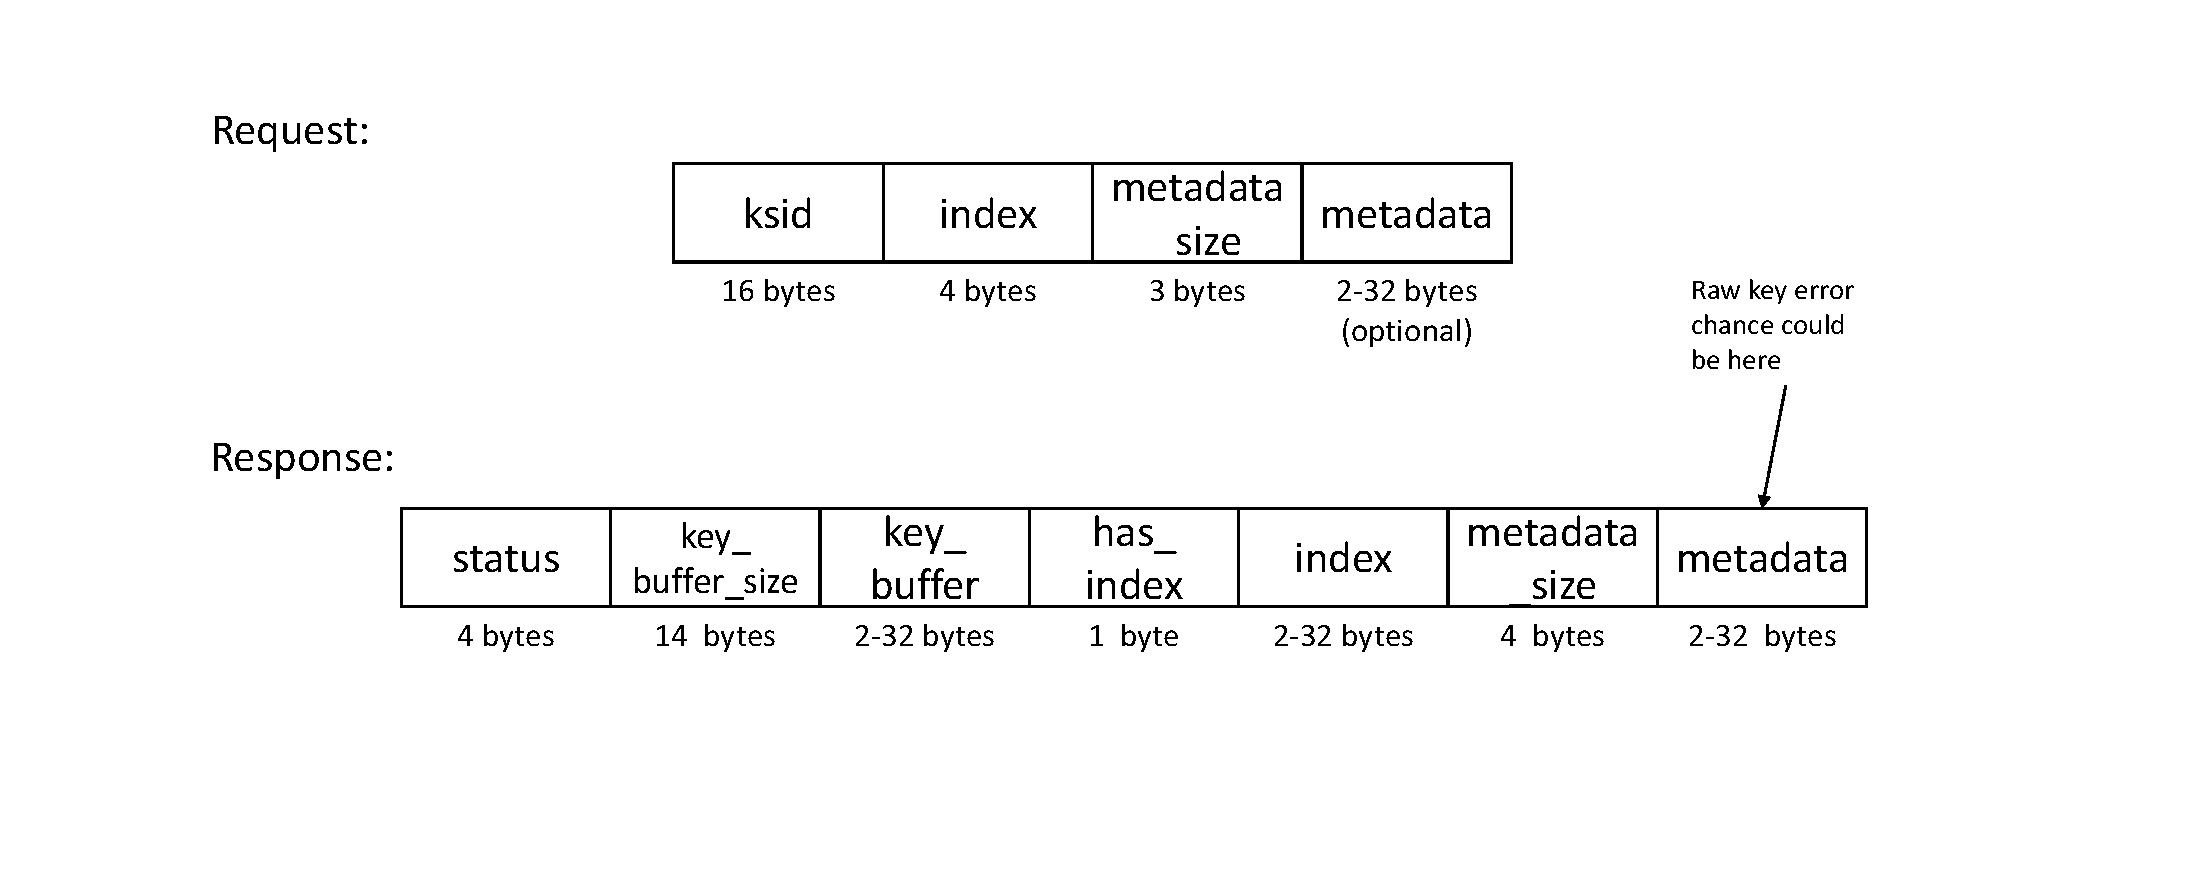
\includegraphics[width=15cm]{get_key_socket.pdf}
	\caption{Get Key Socket}
	\label{fig:getKey}
\end{figure}

\begin{itemize}

	\item\underline{ksid}

		KSID

	\item\underline{index}

		Position of the key to be accessed within the reserved key store for the application

	\item\underline{metadata\textunderscore size}

		Size of the metadata parameter

	\item\underline{metadata}

		Metadata about the key requested/provided

	\item\underline{status}

		Status code returned by the KMS

	\item\underline{key\textunderscore buffer\textunderscore size}

		Size of the key buffer

	\item\underline{key\textunderscore buffer}

		Key Buffer

	\item\underline{has\textunderscore index}

		Field that indicates if the key index is provided

\end{itemize}

\begin{figure}[H]
	\centering
	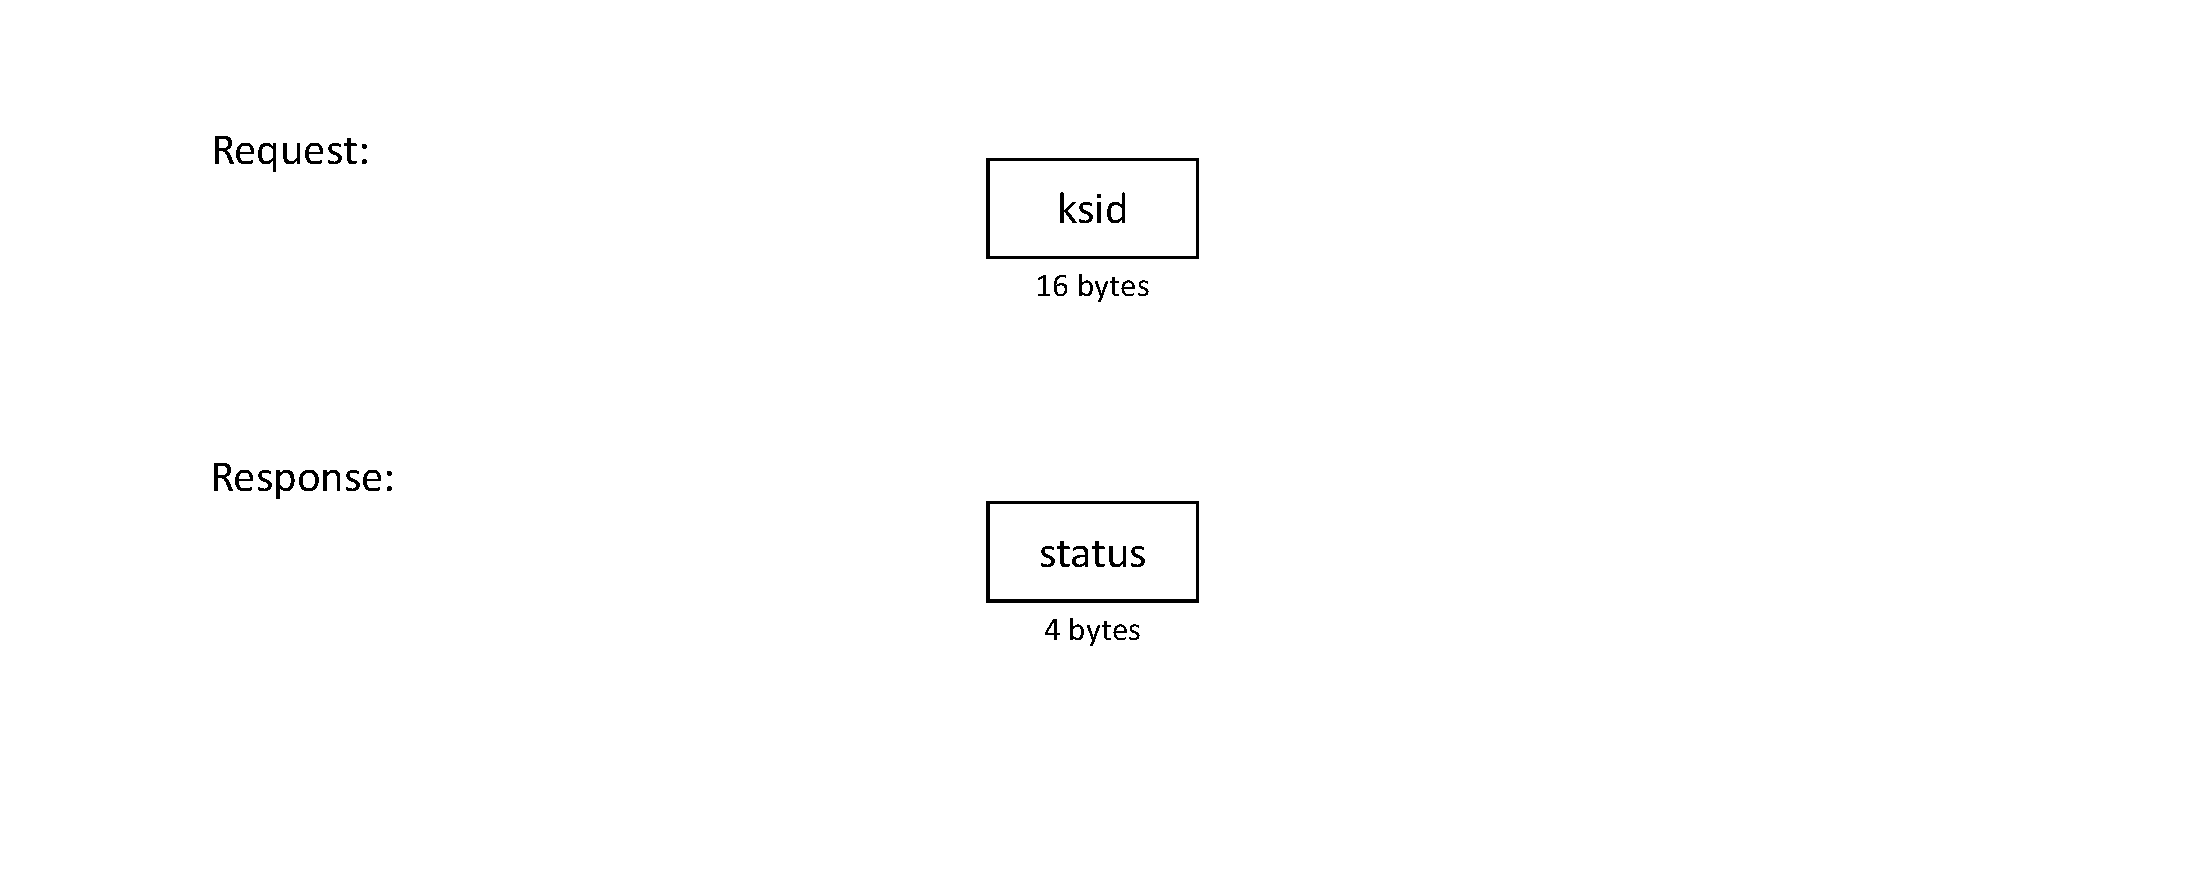
\includegraphics[width=15cm]{close_socket.pdf}
	\caption{Close Socket}
	\label{fig:close}
\end{figure}

\begin{itemize}

	\item\underline{ksid}

		KSID

	\item\underline{status}

		Status code returned by the KMS

\end{itemize}

\subsubsection{Setting up the virtual environment and dependencies}

Before running the example we need to make sure we are using a virtual environment (to have a clean installation), the right python version and the its dependencies.
The first step is to install python 3.6 and gcc, running the following command:

\texttt{sudo apt install -y python3.6-dev gcc virtualenv}

To make sure the right version of python is installed we can run python3 with the --version argument: 

\texttt{python3 --version}

Having python 3.6 installed we can proceed. The next step is to head over to the example directory, \texttt{sdf/etsi\textunderscore qkd\textunderscore 004/madrid\textunderscore example/} and open a terminal there so we can make a virtual environment. To install the virtual environment simply run the command:

\texttt{virtualenv -p python3 qkd004}

This will create a virtual environment with the name \texttt{qkd004}. After installing it we need to activate it. Run the command:

\texttt{source qkd004/bin/activate}

Upon the virtual environment we can install the needed python dependencies by running the command:

\texttt{pip install -r requirements.txt}

At this point, provided there were no errors, everything should be set for running the example.

The scripts should be used inside the virtual environment. After using it, to leave the virtual environment, simply type the command:

\texttt{deactivate}

\subsection{Running the example}

Two run the example simply run the command:

\texttt{python run\textunderscore test.py}

This example will spawn two LKMS and two applications using threads. These applications will exchange messages encrypted with symmetric keys provided by the LMKS.

\begin{figure}[H]
	\centering
	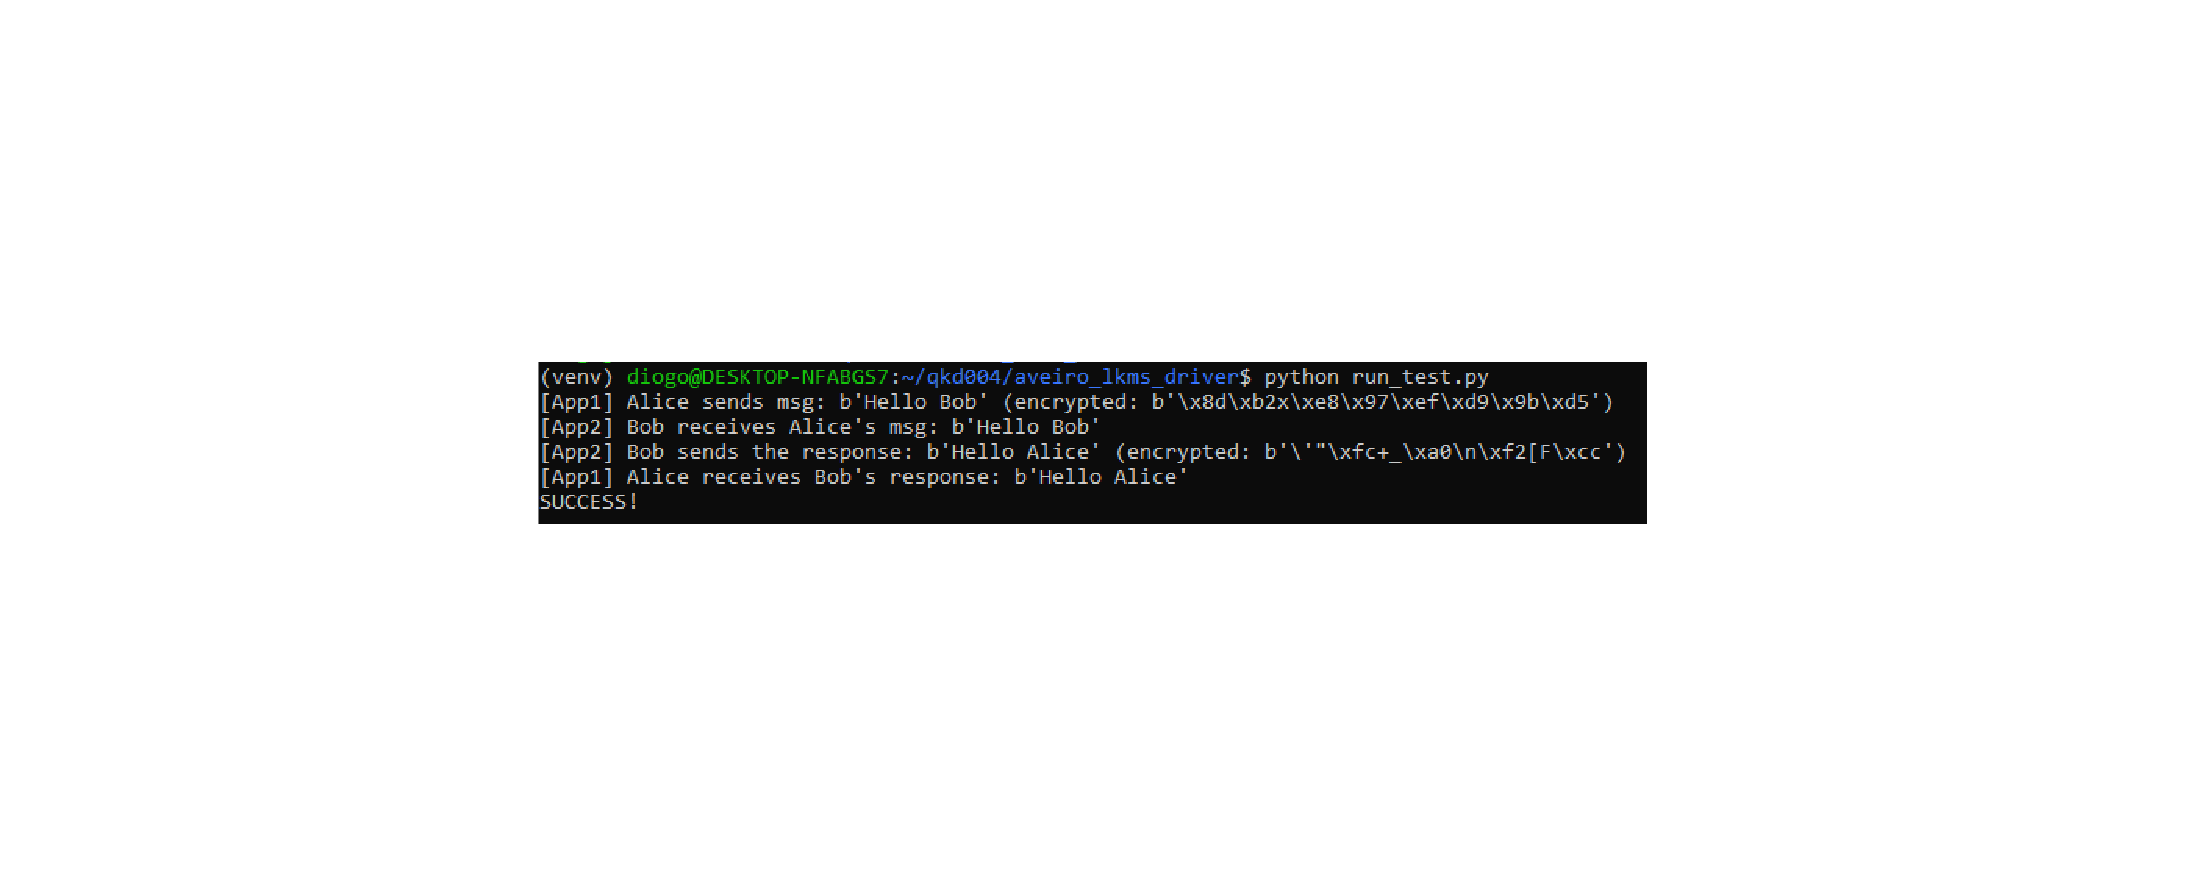
\includegraphics[width=15cm]{madridExample.pdf}
	\caption{Madrid Example}
	\label{fig:madridExample}
\end{figure}

\subsection{Running only two LKMS}

To run the LKMS without running the applications we must first install the qkd004 implementation as a python module by running the following command:

\texttt{pip install etsi\textunderscore qkd\textunderscore 004/}

After that simply run the script \texttt{run\textunderscore lkms.py}:

\texttt{python run\textunderscore lkms.py}

This will spawn two LMKS on separate threads, one in port 44441 and another in port 44442, both on localhost. To change the port or address simply edit lines 5 and 6 of the script.

\subsection{Using the Application driver}

The Madrid example includes a driver for the application. This driver includes functions that implement the socket communication needed to interact with the LMKS API. To use this driver you also need to install the etsi\textunderscore qkd\textunderscore 004 module as described above. Note that you should import the driver at the start of the python script with the following line:

\texttt{from aveiro\textunderscore driver.app\textunderscore 004 import *}

This driver really simplifies the application implementation as there is only the need to initialize the application driver object. From then on if there is the need to encrypt messages just use the encrypt and decrypt method of the application driver.

First declare the variables needed (lkms address, source URI, destination URI and QoS):

\texttt{lkms\textunderscore node1\textunderscore address = ("localhost", 44441)}

\texttt{source = URI("qkd://Application1@aaaaaaaa-aaaa-aaaa-aaaa-aaaaaaaaaaaa")}

\texttt{destination = URI("qkd://Application2@bbbbbbbb-bbbb-bbbb-bbbb-bbbbbbbbbbbb")}

\texttt{qos = QoS(32, 32, 32, 0, 0, 0, 0)}

Being the QoS fields the key\textunderscore chunk\textunderscore size, max\textunderscore bps, min\textunderscore bps, jitter, priority, timeout and ttl, respectively.

Then, to initialize the driver:

\texttt{node1 = App004(lmks\textunderscore node1\textunderscore address, source, destination, qos)}

After that, to encrypt a message simply use:

\texttt{node1.encrypt(message)}

and to decrypt:

\texttt{node1.decrypt(message)}

Note that the message should be in bytes format.

%After cloning the repository the example can be used by running the \texttt{run\textunderscore test.py}. This script launches two LKMS (Light Key Management System) instances and two applications that exchange a encrypted message and then decrypt it using the keys gotten from the QKD.

%The example can also be used to run only the LMKS's by running the script \texttt{run\textunderscore lmks\textunderscore simulator.py} twice. This way we can use the example to test our applications.

%One important note to have in mind is that this example does not have communication between Key Managers, which will need to be implemented in the final Key Manager.

\subsection{Running Alice, Bob and Charlie symmetric key distribution}

There is also an example where 3 parties exchange symmetric keys between each other. This example is present in \texttt{sdf/etsi\textunderscore qkd\textunderscore 004/qkd004/}. To run this example simply set up the virtual environment and dependencies like explained before and run (in this order):

In Alice:

\texttt{python3 run\textunderscore alice.py}

In Bob:

\texttt{python3 run\textunderscore bob.py aliceIP}, using alice's IP address as argument

In Charlie:

\texttt{python3 run\textunderscore charlie.py aliceIP bobIP}, replacing with Alice's and Bob's IP

You should see in each computer an exchange of message between peers.

\begin{figure}[H]
	\centering
	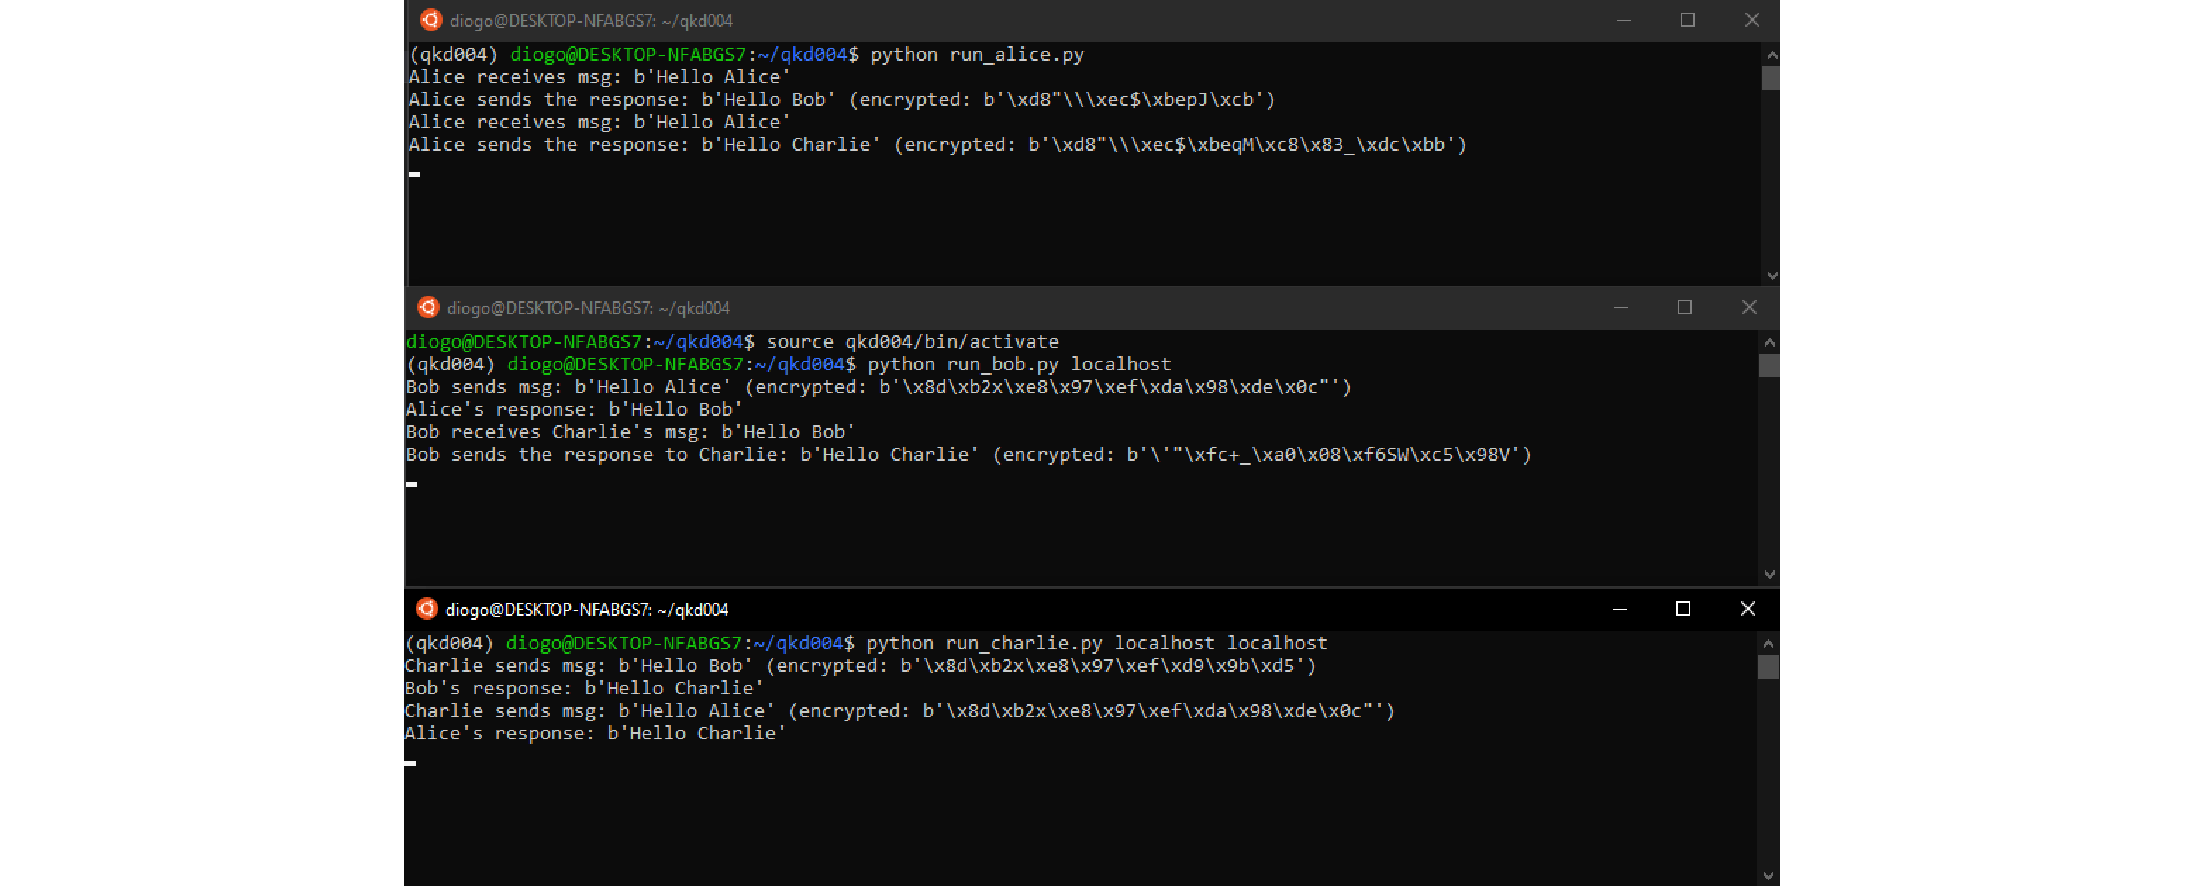
\includegraphics[width=15cm]{alicebobcharlie_example.pdf}
	\caption{Running the examples all on the same machine}
	\label{fig:3partyexample}
\end{figure}

\subsection{Raw Key Distribution}

\begin{figure}[H]
	\centering
	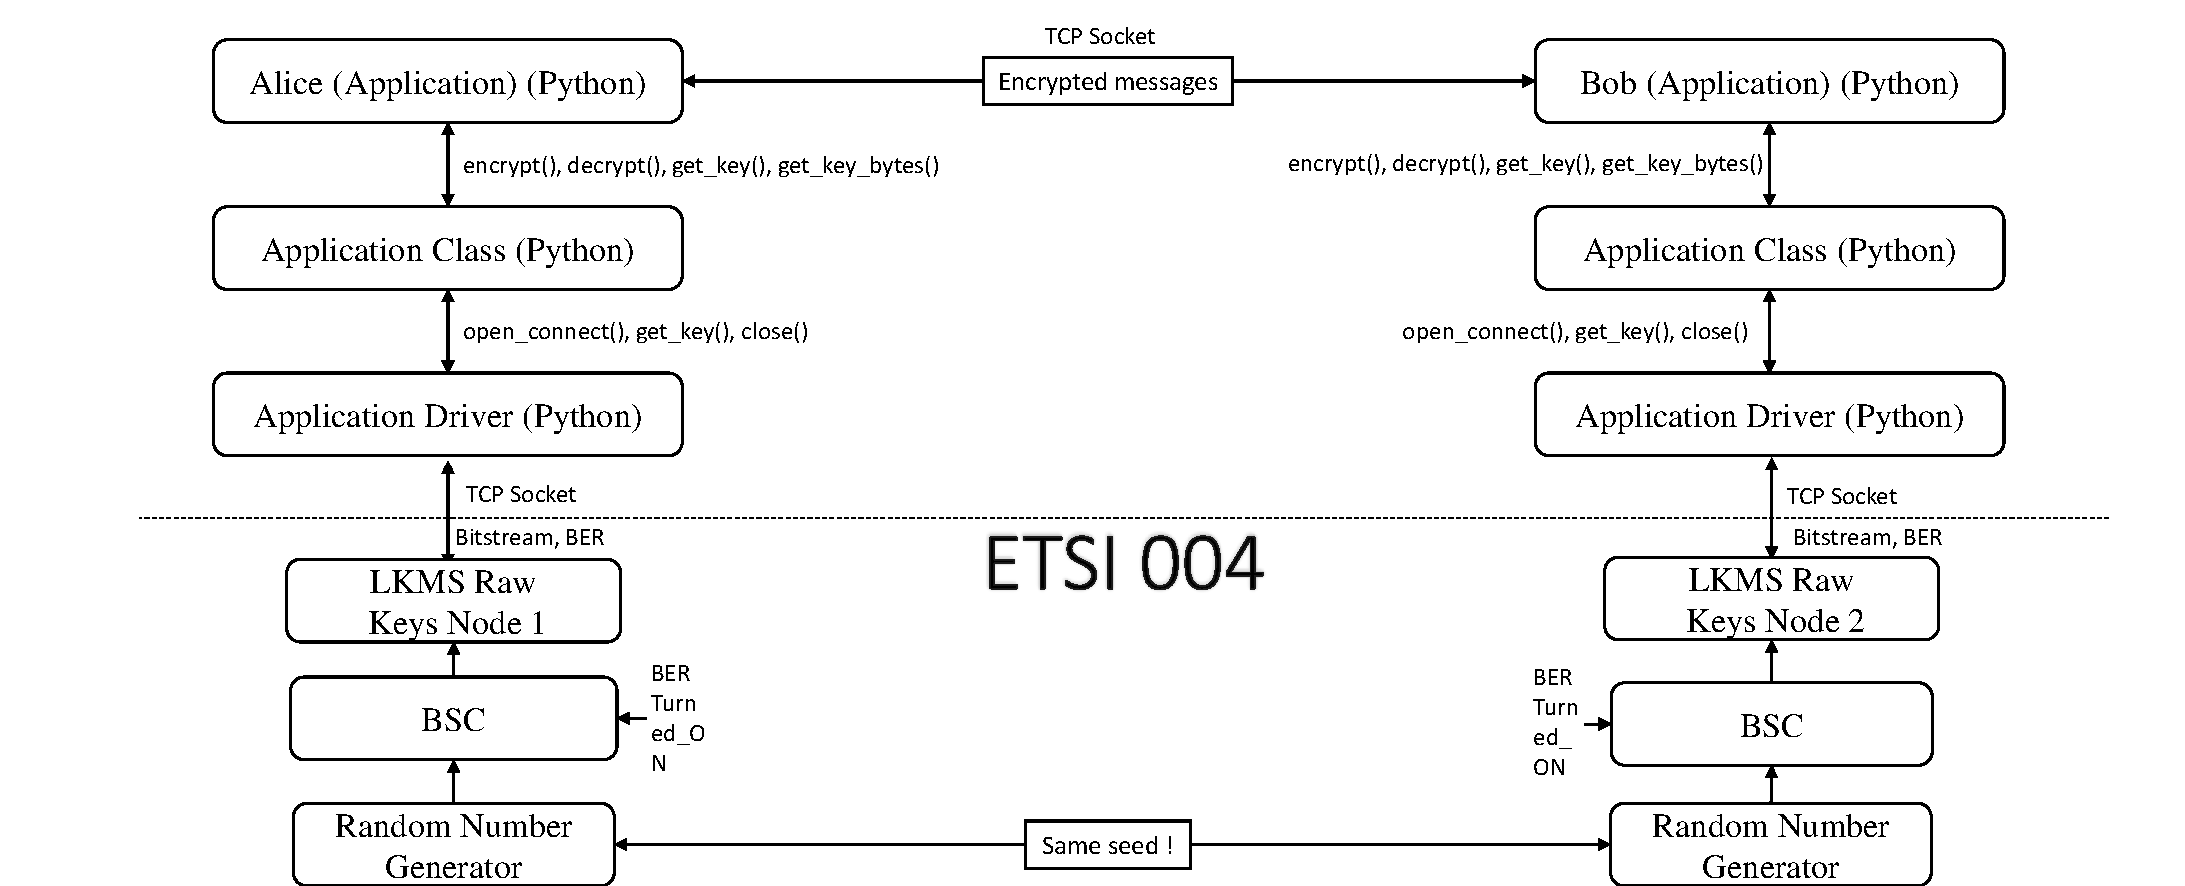
\includegraphics[width=15cm]{raw_key_distribution.pdf}
	\caption{Raw Key Distribution}
	\label{fig:rawkeydistribution}
\end{figure}

We have adapted the Madrid QKD example to also distribute raw keys. The way it works is when the LKMS Simulator is deployed, a seed and an error chance is associated with it. To deploy the LMKS use the following function:

\texttt{LKMSSimulator(("Address",Port),Seed,Error\textunderscore chance)}

The error chance should be an integer from 0 to 100

To connect to the Raw Key Manager you should use the same procedure as the symmetric key manager:

\texttt{app004 = App004(lkms\textunderscore address, source, destination, qos, KeyStreamId)}

The key can then be retrieved with:

\texttt{key = app004.get\textunderscore key\textunderscore bytes(size)}

An example called "test\textunderscore raw\textunderscore keys.py" is available in \texttt{/sdf/etsi\textunderscore qkd\textunderscore 004/qkd004/} 

\subsection{Development plan}

\begin{itemize}
	
	\item\underline{Socket Driver}

		Develop the socket driver, responsible for translating the API functions into bytes and parsing its responses.
		
		Classes:
		\begin{itemize}
			\item\underline{ksid}
			\item\underline{uri}
			\item\underline{qos}
			\item\underline{key\textunderscore buffer}
			\item\underline{metadata}
		\end{itemize}				
		
		Functions:
		\begin{itemize}
			\item\underline{openConnectRequest\textunderscore tobytes}
			\item\underline{openConnectRequest\textunderscore frombytes}
			\item\underline{openConnectResponse\textunderscore tobytes}
			\item\underline{openConnectResponse\textunderscore frombytes}
			\item\underline{getKeyRequest\textunderscore tobytes}
			\item\underline{getKeyRequest\textunderscore frombytes}
			\item\underline{getKeyResponse\textunderscore tobytes}
			\item\underline{getKeyResponse\textunderscore frombytes}
			\item\underline{closeRequest\textunderscore tobytes}
			\item\underline{closeRequest\textunderscore frombytes}
			\item\underline{closeResponse\textunderscore tobytes}
			\item\underline{closeResponse\textunderscore frombytes}
		\end{itemize}
	
	\item\underline{Application-KMS Driver Class}
		
		Create an Application driver class, responsible for storing and managing important information like QoS and KSID that can be used in its calls to the API using the Socket Driver.
		
		Attributes:
		\begin{itemize}
			\item\underline{kms\textunderscore address}
		\end{itemize}
		
		Methods:
		\begin{itemize}
		
			\item\underline{KmsDriver(address)}
		
				Application-Kms driver constructor	
		
			\item\underline{~KmsDriver}
		
				Application-Kms driver destructor
		
			\item\underline{void open\textunderscore connect(source, destination, qos, ksid, status)}
		
				Open Connect function
		
			\item\underline{void get\textunderscore key(ksid, index, metadata, status, key\textunderscore buffer)}
		
				Get Key function
		
			\item\underline{void close(ksid,status)}
		
				Close function
		
		\end{itemize}
		
	\item\underline{Application Class}
	
		Create an Application Class, responsible for abstracting the programmer from inner workings of the ETSI protocol, enabling him to provide the parameters and get the Key Buffer in return.
		
		Attributes:
		\begin{itemize}
			\item\underline{source}
			\item\underline{destination}
			\item\underline{qos}
			\item\underline{ksid}
			\item\underline{index}
			\item\underline{key\textunderscore buffer}
		\end{itemize}
		
		Methods:
		\begin{itemize}
			
			\item\underline{App004(address, source, destination, qos, ksid)}
		
				Application Class constructor	
		
			\item\underline{~App004}
		
				Application Class destructor
		
			\item\underline{keyBuffer get\textunderscore key(int size)}
		
				Gets key buffer as a KeyBuffer object
		
			\item\underline{char* get\textunderscore key\textunderscore bytes(int size)}
		
				Gets key buffer as an array of bytes
		
			\item\underline{char* encrypt(char* message)}
		
				Encrypts a message using XOR method
		
			\item\underline{char* decrypt(char* message)}
		
				Decrypts a message using XOR method
		
	\end{itemize}

	Example: 
	\begin{verbatim}
	#include <iostream>
	#include <string>
	#include "app_class.h"
	
	int main(){
		
		// LKMS Address and port
		
		std::string lkms_address = "192.168.1.100";
		uint32_t lkms_port = 44440;
		
		// Source and destination URI
		
		std::string source_uri =
		 "qkd://Application1@aaaaaaaa-aaaa-aaaa-aaaa-aaaaaaaaaaaa";
		std::string destination_uri =
		 "qkd://Application2@bbbbbbbb-bbbb-bbbb-bbbb-bbbbbbbbbbbb";
		
		// QoS - key_chunk_size, max_bps, min_bps, jitter, priority, ttl,
		// metadata_mimetype
		
		QoS qos = QoS(32,32,32,0,0,0,"raw+oblivious");
		
		// KSID
		
		std::string ksid = "12345678-1234-1234-1234-123456789012";
		
		// Initialize App class
		
		App004 alice_app = App004(lkms_address, lkms_port, source_uri,
		 destination_uri, qos, ksid);
		
		// Request a key from the App class
		
		char* key_buffer = alice_app.get_key_bytes(20, RAW_KEY);
		
		// Close connection
		
		alice_app.close()
		
	}		
	\end{verbatim}
	
		
\end{itemize}

\subsection{Madrid cpp 004 example}

\subsubsection{Introduction}

\begin{figure}[H]
	\centering
	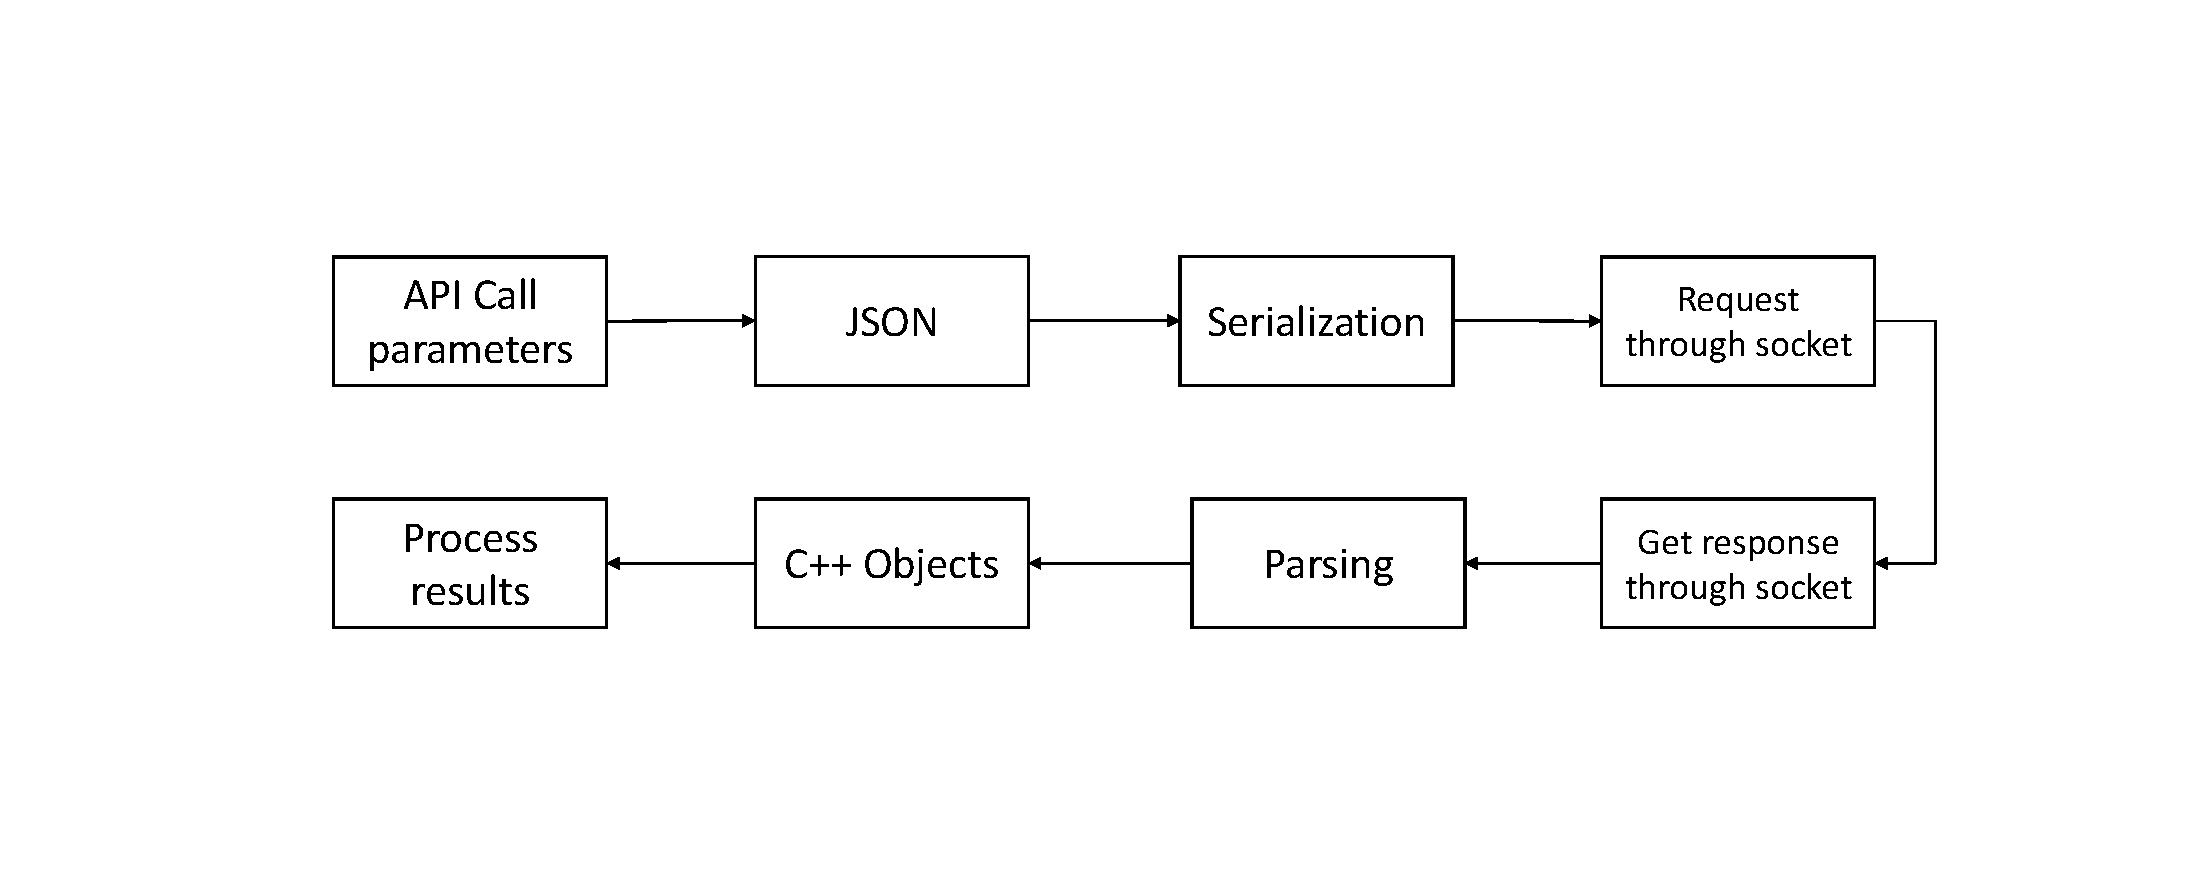
\includegraphics[width=15cm]{madrid_cpp.pdf}
	\caption{Madrid cpp example}
	\label{fig:madridcpp}
\end{figure}

The figure above tries to ilustrate how the cpp madrid example works. To start the API call parameters are defined. Once those parameters are defined (by the user), the API call function can be called. This function procedes to convert these parameters into a JSON object. The JSON object is then serialized and sent through a socket to the KMS. A response should be sent from the KMS through that same socket, which is then parsed and converted into a response struct and returned to the user that can then interpret these results as he wishes to.

\subsubsection{Example}

An example on how to use the madrid 004 cpp library was provided:

\begin{verbatim}
	#include <iostream>
	#include <nlohmann/json.hpp>
	#include "etsi_qkd_004.hpp"
	#include <stdexcept>
	#include <thread>
	
	void print_key_buffer(const etsi_qkd_004::KeyBuffer& key_buffer, 
	const std::string& name = "KEY BUFFER") {
		std::cout << name << ": [ ";
		std::for_each(key_buffer.cbegin(), key_buffer.cend(), 
		[](const unsigned char &c) { 
			std::cout << int(c) << " "; });
		std::cout << "]" << std::endl;
	}
	
	
	int main(int argc, char **argv) {
		if (argc - 1 != 2)
		throw std::invalid_argument("ERROR: Number of arguments " +
		std::to_string(argc - 1) +
		"\narg1 should be IP (ex: \"127.0.0.1\")"
		"\narg2 should be the PORT (ex: 1234)\n");
		
		etsi_qkd_004::LKMSAddress address = {argv[1], (unsigned short) atoi(argv[2])};
		std::cout << "Using address: " << address.ip << ':' 
		<< address.port << std::endl;
		
		// CONFIGURE DESIRED KEY (CHUNK_SIZE * CHUNK_NUMBER in bytes)
		// Number of key bytes retrieved per GET_KEY
		const unsigned int CHUNK_SIZE = 5;  
		// Number of key chunks you want to get
		const unsigned int CHUNK_NUMBER = 8;  
		
		// ----- OPEN_CONNECT -----
		// Classic key
		//    std::string source = "qkd:Application2@cccccccc-cccc-cccc-cccc-cccccccccccc";  
		// Classic key
		//    std::string destination = "qkd:Application1@bbbbbbbb-bbbb-bbbb-bbbb-bbbbbbbbbbbb";  
		// Raw key
		std::string source = "raw:Application2@cccccccc-cccc-cccc-cccc-cccccccccccc";  
		// Raw key
		std::string destination = "raw:Application1@bbbbbbbb-bbbb-bbbb-bbbb-bbbbbbbbbbbb";  
		
		etsi_qkd_004::QoS qos = {CHUNK_SIZE, 32, 32, 0, 0, 150000, 0, ""};
		auto oc_response = etsi_qkd_004::open_connect(address, 
		source, destination, qos);
		std::cout << "OPEN CONNECT STATUS: " << oc_response.status << std::endl;
		
		// ----- GET_KEY -----
		etsi_qkd_004::KeyBuffer cumulative_key_buffer;
		unsigned int index = 0;
		while (index < CHUNK_NUMBER) {
			std::this_thread::sleep_for(std::chrono::milliseconds(1000));
			auto gk_response = etsi_qkd_004::get_key(address, 
			oc_response.key_stream_id, index);
			if (gk_response.status == etsi_qkd_004::Status::SUCCESSFUL) {
				print_key_buffer(gk_response.key_buffer);
				
				// Extend cumulative_key_buffer
				cumulative_key_buffer.reserve(cumulative_key_buffer.size() +
				std::distance(gk_response.key_buffer.cbegin(),
				gk_response.key_buffer.cend()));
				cumulative_key_buffer.insert(cumulative_key_buffer.cend(),
				 gk_response.key_buffer.cbegin(),
				gk_response.key_buffer.cend());
				// Increment chunk index (only if gk_response.status is SUCCESSFUL)
				++index;
			}
			else
			;//std::cout << "ERROR: Status " << gk_response.status << std::endl;
		}
		print_key_buffer(cumulative_key_buffer, "CUMULATIVE KEY BUFFER");
		
		// ----- CLOSE -----
		auto cl_response = etsi_qkd_004::close(address, oc_response.key_stream_id);
		std::cout << "CLOSE STATUS: " << cl_response.status << std::endl;
		
		
		return 0;
	}
	
\end{verbatim}

This example can be found at sdf/etsi\textunderscore qkd\textunderscore 004/cpp/ .

It is important to note that the type of key requested is defined by the scheme in the URI.

To compile it use cmake:

\begin{verbatim}
	sudo apt-get install uuid-dev build-essential libssl-dev
	sudo snap install cmake --classic
	mkdir cmake-build
	cd cmake-build
	cmake ..
\end{verbatim}

\subsection{Requesting keys}

The type of keys requested are defined by the scheme in the URI. Example of QOKD URI: \texttt{"qokd:Application2@cccccccc-cccc-cccc-cccc-cccccccccccc"}.

Sample bytes received:

Alice: 10 10 10 00


Bob: 01 01 01 00

The first bit is the selection byte and the second one is the corresponding bit. 

To change the role played in QOKD use the role parameter in open\textunderscore connect. Example:

\begin{verbatim}
	std::string role = "bob";
	auto oc_response = etsi_qkd_004::open_connect(address, source, destination, qos,"b0dd24e6-94cb-4f32-abfe-50e194783a48", role);
\end{verbatim}


The system also provides symmetrical and raw keys:

\texttt{"qkd:Application2@cccccccc-cccc-cccc-cccc-cccccccccccc"}
\texttt{"raw:Application2@cccccccc-cccc-cccc-cccc-cccccccccccc"}


\subsection{Changing raw bit error rate}

To change the LKMS error rate edit the second parameter of LKMSSimulator on /sdf/etsi\textunderscore qkd\textunderscore 004/lkms/run\textunderscore lkms.py :

\begin{verbatim}
	def run_lkms_simulator(lkms_address):
		LKMSSimulator(lkms_address, 50)
\end{verbatim}


In this example the bit error rate is set to 50%

\subsection{How to get QKD, QOKD and RAW keys}

For the key delivery service to work we need two parts: the LKMS (Key Management Service) and the client.
The LKMS generates a different set of keys for each KSID (with the correct type, specified by the user). 
To start the LKMS execute \texttt{python3 run\textunderscore lkms.py} at \texttt{/sdf/etsi\textunderscore qkd\textunderscore 004/lkms/}. If you want to change the raw key error rate open 
the run\textunderscore lkms.py script and change the second argument of LKMSSimulator. Example of 50% error rate: 
\begin{verbatim}
	def run_lkms_simulator(lkms_address):
		LKMSSimulator(lkms_address, 50)
\end{verbatim}

After starting the LKMS Simulator it should be ready to provide keys. To test this you can use the example cpp program or write your own. The program is located in \texttt{/sdf/etsi\textunderscore qkd\textunderscore 004/cpp/}. If all is working then the cpp program should print out the keys provided by the LKMS. There are a couple of things that can be changed in the program:

\begin{itemize}
	\item\underline{KSID}
		You can provide your own KSID. In case you don't the LKMS should generate one and return it on the open\textunderscore connect call.

	\item\underline{Type of keys}
		The type of keys provided depends on the scheme of the source URI. Example:

		\texttt{"qkd:Application2@cccccccc-cccc-cccc-cccc-cccccccccccc"}
		\texttt{"raw:Application2@cccccccc-cccc-cccc-cccc-cccccccccccc"}

		The first one provides qkd keys and the second on raw. There are also qokd keys.

	\item\underline{Role of qokd keys}	

		To change the role (alice or bob) when getting qokd keys add a argument to the open\textunderscore connect function:

		\begin{verbatim}
			std::string role = "bob";
			auto oc_response = etsi_qkd_004::open_connect(address, source, destination
, qos,"b0dd24e6-94cb-4f32-abfe-50e194783a48", role);
		\end{verbatim}


\end{itemize}

To compile the example you first need to install the dependencies:
\begin{verbatim}
	sudo apt-get install uuid-dev build-essential libssl-dev
	sudo snap install cmake --classic
\end{verbatim}

After that go to the folder of the example:
\begin{verbatim}
mkdir cmake-build
cd cmake-build
cmake ..
make
\end{verbatim}
\subsection{Further Discussion}

\subsection{Open Issues}

\subsection{References}

\begin{itemize}
	\item
		ETSI GS QKD 004 V2.1.1 (2020-08)
\end{itemize}




\pagebreak


%%%%%%%%%%%%%%%%%%%%%%%%%%%%%%%%%%%%%%%%%%%%%%%%%%%%%%%%%%%%%%%%%%%%%%%%%%%%%%%%
% Acronyms
%%%%%%%%%%%%%%%%%%%%%%%%%%%%%%%%%%%%%%%%%%%%%%%%%%%%%%%%%%%%%%%%%%%%%%%%%%%%%%%%
\clearpage
\subsection*{Acronyms}\label{sec:acronyms}
\begin{acronym}[TDMA]
	\acro{DV-QKD}[DV-QKD]{Discrete Variables Quantum Key Distribution}
	\acro{QKD}[QKD]{Quantum Key Distribution}
\end{acronym}
\pagebreak 

%%%%%%%%%%%%%%%%%%%%%%%%%%%%%%%%%%%%%%%%%%%%%%%%%%%%%%%%%%%%%%%%%%%%%%%%%%%%%%%%
% References
%%%%%%%%%%%%%%%%%%%%%%%%%%%%%%%%%%%%%%%%%%%%%%%%%%%%%%%%%%%%%%%%%%%%%%%%%%%%%%%%

% bibliographic references for the section ----------------------------
\clearpage
\printbibliography[heading=subbibliography]
\end{refsection}
\addcontentsline{toc}{subsection}{Bibliography}
\cleardoublepage
% ---------------------------------------------------------------------

